
%(BEGIN_QUESTION)
% Copyright 2013, Tony R. Kuphaldt, released under the Creative Commons Attribution License (v 1.0)
% This means you may do almost anything with this work of mine, so long as you give me proper credit

Examine this process trend showing the PV, SP, and Output of a loop controller:

$$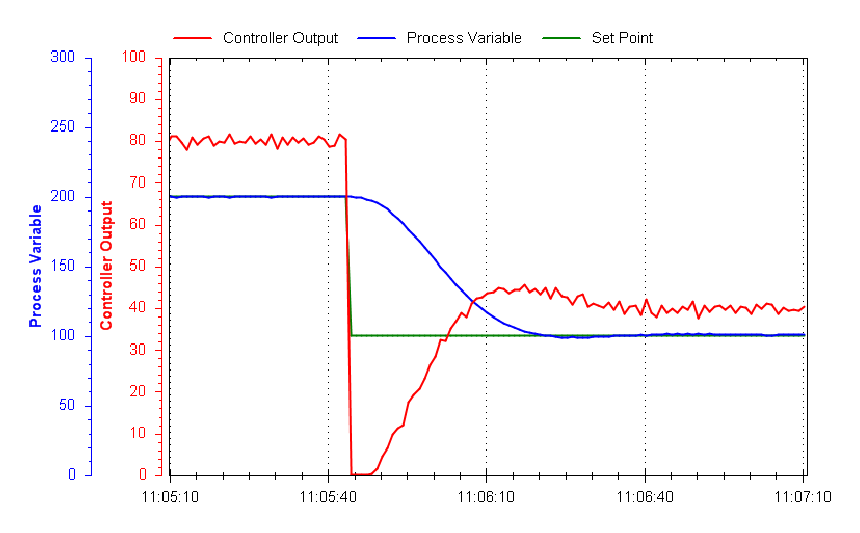
\includegraphics[width=15.5cm]{i02644x01.eps}$$

Based on what you see here, determine the following:

\begin{itemize}
\item{} Whether this is an open-loop or a closed-loop response
\item{} Whether the controller is (or needs to be) {\it direct-acting} or {\it reverse-acting}
\item{} If possible, identify any problems with the field instrumentation
\item{} If possible, identify any problems with the controller PID tuning
\item{} Qualitatively identify the kind of PID tuning we will need for robust control
\end{itemize}

\underbar{file i02644}
%(END_QUESTION)





%(BEGIN_ANSWER)

This is a {\it closed-loop test}, based on the fact the output signal responds dynamically to the changing process variable, as well as to the step-change in setpoint.

\vskip 10pt

This is a {\it reverse-acting} controller: the output steps down when the setpoint steps down (implying the output would step down if the process variable stepped up).

\vskip 10pt

There do not appear to be any field instrumentation problems revealed in this trend.  We can see some multiple-order lag time, but this is not necessarily an instrument problem. 

\vskip 10pt
  
The controller tuning is actually quite good.  The only possible criticism here is that the output trend is a bit noisy, which if controlling a valve may cause the valve to move excessively (using more compressed air than is necessary, and wearing out the packing).

\vskip 10pt

This is clearly a self-regulating process with multiple orders of lag.  Ordinarily, some derivative action will help permit more aggressive proportional and integral actions that would otherwise be possible with a P+I controller, but here with the noise problem we may have to be careful how much derivative action we put into this loop controller.  As was mentioned earlier, the tuning in this loop is actually quite good.

%(END_ANSWER)





%(BEGIN_NOTES)


%INDEX% Process troubleshooting: diagnosing problem via trend recording

%(END_NOTES)


